%%%%%%%%%%%%%%%%%%%%%%%%%%%%%%%%%%%%%%%%%
% Short Sectioned Assignment LaTeX Template Version 1.0 (5/5/12)
% This template has been downloaded from: http://www.LaTeXTemplates.com
% Original author:  Frits Wenneker (http://www.howtotex.com)
% License: CC BY-NC-SA 3.0 (http://creativecommons.org/licenses/by-nc-sa/3.0/)
%%%%%%%%%%%%%%%%%%%%%%%%%%%%%%%%%%%%%%%%%

%----------------------------------------------------------------------------------------
%	PACKAGES AND OTHER DOCUMENT CONFIGURATIONS
%----------------------------------------------------------------------------------------

\documentclass[paper=a4, fontsize=11pt]{scrartcl} % A4 paper and 11pt font size

% ---- Entrada y salida de texto -----

\usepackage[T1]{fontenc} % Use 8-bit encoding that has 256 glyphs
\usepackage[utf8]{inputenc}
%\usepackage{fourier} % Use the Adobe Utopia font for the document - comment this line to return to the LaTeX default

% ---- Idioma --------

\usepackage[spanish, es-tabla]{babel} % Selecciona el español para palabras introducidas automáticamente, p.ej. "septiembre" en la fecha y especifica que se use la palabra Tabla en vez de Cuadro

% ---- Otros paquetes ----

\usepackage{url} % ,href} %para incluir URLs e hipervínculos dentro del texto (aunque hay que instalar href)
\usepackage{amsmath,amsfonts,amsthm} % Math packages
%\usepackage{graphics,graphicx, floatrow} %para incluir imágenes y notas en las imágenes
\usepackage{graphics,graphicx, float} %para incluir imágenes y colocarlas

% Para hacer tablas comlejas
%\usepackage{multirow}
%\usepackage{threeparttable}

%\usepackage{sectsty} % Allows customizing section commands
%\allsectionsfont{\centering \normalfont\scshape} % Make all sections centered, the default font and small caps

\usepackage{fancyhdr} % Custom headers and footers
\pagestyle{fancyplain} % Makes all pages in the document conform to the custom headers and footers
\fancyhead{} % No page header - if you want one, create it in the same way as the footers below
\fancyfoot[L]{} % Empty left footer
\fancyfoot[C]{} % Empty center footer
\fancyfoot[R]{\thepage} % Page numbering for right footer
\renewcommand{\headrulewidth}{0pt} % Remove header underlines
\renewcommand{\footrulewidth}{0pt} % Remove footer underlines
\setlength{\headheight}{13.6pt} % Customize the height of the header

\numberwithin{equation}{section} % Number equations within sections (i.e. 1.1, 1.2, 2.1, 2.2 instead of 1, 2, 3, 4)
\numberwithin{figure}{section} % Number figures within sections (i.e. 1.1, 1.2, 2.1, 2.2 instead of 1, 2, 3, 4)
\numberwithin{table}{section} % Number tables within sections (i.e. 1.1, 1.2, 2.1, 2.2 instead of 1, 2, 3, 4)

\setlength\parindent{0pt} % Removes all indentation from paragraphs - comment this line for an assignment with lots of text

\newcommand{\horrule}[1]{\rule{\linewidth}{#1}} % Create horizontal rule command with 1 argument of height

%----------------------------------------------------------------------------------------
%       TÍTULO Y DATOS DEL ALUMNO
%----------------------------------------------------------------------------------------
\usepackage{cite}
\usepackage{hyperref}
\usepackage{titlesec}
\title{ 
\normalfont \normalsize 
\textsc{\textbf{Ingeniería de Redes (2016-2017)} \\ Grado en Ingeniería Informática \\ Universidad de Granada} \\ [25pt] % Your university, school and/or department name(s)
\horrule{0.5pt} \\[0.4cm] % Thin top horizontal rule
\huge Trabajo de ingeniería de redes \\ % The assignment title
\horrule{2pt} \\[0.5cm] % Thick bottom horizontal rule
}
\author{Javier Oliva Cruz y Javier Gómez Luzón} % Nombre y apellidos
\date{29/10/2016} % Incluye la fecha actual
\newpage
%----------------------------------------------------------------------------------------
% DOCUMENTO
%----------------------------------------------------------------------------------------
\begin{document}
\maketitle
\pagebreak
\tableofcontents
\listoffigures
\pagebreak
\section{Introducción a SPDY}
\subsection{¿Qué es SPDY?}
SPDY es un protocolo de transporte diseñado como un sucesor de HTTP, desarrollado por un equipo que incluye ingenieros encargados en la creación de otros protocolos como HTTP/2, este protocolo nace a partir de la experimentación de protocolos alternativos que ayuden a reducir la latencia de las páginas web. SPDY es un protocolo que se beneficia del código abierto, la comunidad contribuye con ideas, código y resultados de test para hacer que SPDY sea el protocolo más rápido de la siguiente generación. A día de hoy SPDY reduce el tiempo de carga respecto a HTTP en alrededor de un 64\%.
\\
\subsection{Definiciónes}
\begin{itemize}
\item \textbf{Clientes:} Es el endpoint que inicia la sesion SPDY.
\item \textbf{Conexión:} El transporte entre dos endpoints.
\item \textbf{Endpoint:} El cliente o el servidor de una conexión.
\item \textbf{Frame:} Una cabecera prefijada por una secuencia de bytes enviada a través de una sesión de SPDY.
\item \textbf{Servidor:} El endpoint que no inicializa la sesión SPDY.
\item \textbf{Stream:} flujo bidireccional de bytes a traves de un canal virtual en una sesión de SPDY.
\end{itemize}

\subsection{HTTP y sus principales problemas}
Para entender mejor las ventajas del protocolo SPDY hace falta entender también a HTTP y los problemas que este tiene.
HTTP (Hypertext Transfer Protocol) es un protocolo de transacción de datos con el esquema cliente-servidor que se usa para la entrega de archivos y otros datos llamados ‘mensajes’.
Los mensajes HTTP son un texto plano, lo que los hace más legibles y fáciles de depurar, lo que conlleva que estos mensajes sean más largos. Los mensajes siguen la estructura de:
\begin{itemize}
\item \textbf{Línea inicial}

\item \textbf{Cabecera} 

\item \textbf{Cuerpo del mensaje.} El cual es opcional
\end{itemize}
HTTP cuenta con una serie de “problemas” que nos obliga a buscar unos protocolos alternativos. Una de ellas es el cuello de botella que ocurre en HTTP es que solo se basa en múltiples conexiones concurrentes. Esto causa varios problemas que el HTTP “pipelining” no soluciona, ya que la conexión puede ser bloqueada en la solicitud de la línea de la cabecera.
Además, muchos proxies tienen un mal soporte para el pipelining.

\subsection{Principales diferencias entre SPDY y HTTP}
SPDY pretende abordar esto y otros problemas relacionados con las web modernas, usando tres mejoras básicas respecto a HTTP:
\begin{itemize}
\item \textbf{Cabeceras comprimidas.} Los clientes actuales envían una gran cantidad de datos redundantes en las cabeceras de los HTTP, porque una sola página web puede requerir entre 50 o 100 subsolitudes. Comprimiendo las cabeceras conseguimos reducir la latencia y ancho de banda que se requiere comparado con HTTP.
\item \textbf{Solicitudes multiplexadas.}  No hay límite para el número de solicitudes que pueden ser emitidas concurrentemente en una sola conexión SPDY, ya que las solicitudes pueden ser intercaladas en un solo canal, la eficiencia del TCP es mucho más alta.
\item \textbf{Priorizar solicitudes.} Los clientes pueden solicitar que recurso se les entregará primero. Con esto evitamos problemas  de atasco en la red provocados por solicitudes no críticas que obstaculizan aquellas con mayor prioridad.
\end{itemize}

\section{¿Cómo se conecta SPDY?}
Para las conexiones SPDY utiliza el protocolo de transporte TCP,  con este las aplicaciones pueden conectarse de manera segura independientemente de las capas inferiores, lo que significa que los router solo tienen que enviar los datos en forma de datagrama. Para cumplir con un buen rendimiento, se espera que los clientes no cierren las conexiones abiertas hasta que el usuario salga de todas las web o hasta que el servidor cierre la conexión. 
\\
Los servidores están encargados de dejar la conexión abierta tanto como sea posible, pero pueden cerrar conexiones ociosas en el caso de que sea necesario.
\\
Cuando cualquier endpoint cierre la conexión con el nivel de transporte, debe en primer lugar mandar un GOAWAY frame con lo que los endpoints pueden determinar si requiere finalizar la conexión antes de cerrarla.

\section{Funcionamiento del framing}
Una vez se establece la conexión, los clientes y servidores intercambian mensajes a través de 2 frames.
\begin{itemize}
\item \textbf{Control\_frames.}
\item \textbf{Data\_frames.}
\end{itemize}
Estos frames mantienen una serie de características comunes, que explicaremos a continuación.

\subsection{Control\_ frames}
\begin{figure}[H] %con el [H] le obligamos a situar aquí la figura
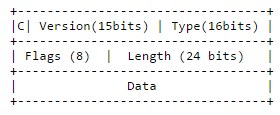
\includegraphics[scale=1]{controlframes.png}  %el parámetro scale permite agrandar o achicar la imagen. En el nombre de archivo puede especificar directorios
\centering
\caption{Estructura del control\_frames} \label{fig:figura1}
\end{figure}
\begin{itemize}
\item \textbf{Bit de control:} La ‘C’ es un solo bit que indica si este es un mensaje de control. Para los frames de control este valor es siempre 1.
\item \textbf{Versión:}  El número de versión del protocolo SPDY.Su tamaño es de 15 bits.
\item \textbf{tipo:} Es el tipo de control\_frame.
\item \textbf{Flags:} Sus flags son diferentes a los que tienen los data\_frames.
\item \textbf{Longitud:} Un valor de 24 bits representando el número de bytes de la longitud del campo.
\item \textbf{Data:} El formato y longitud de estos datos está controlado por  Type.
\end{itemize}
\textbf{Requerimientos del control\_frame:}

La longitud completa de los control\_frame son de 16MB, pueden ser grandes para las implementaciones con recursos limitados. En estos casos, las implementaciones pueden limitar el marco de la longitud máxima admitida. Sin embargo, todas las implementaciones deben ser capaz de recibir frames de control de al menos 256 bytes.

\subsection{Data\_frames}
\begin{figure}[H] %con el [H] le obligamos a situar aquí la figura
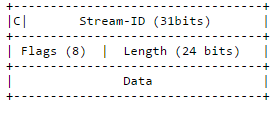
\includegraphics[scale=1]{dataframes.png}  %el parámetro scale permite agrandar o achicar la imagen. En el nombre de archivo puede especificar directorios
\centering
\caption{Estructura del Data\_frames} \label{fig:figura2}
\end{figure}
\begin{itemize}
\item \textbf{Bit de control:} Será siempre 0.
\item \textbf{Stream-ID:} Un valor de que identifica al stream de 31 bits.
\item \textbf{Flags:} Solo tiene un flag (0x01 =FLAG\_FIN - indica que este marco representa la última trama a transmitir en esta corriente).
\item \textbf{Length:} Un valor de 24 bits sin signo que representa el número de bytes después del campo de longitud. El tamaño total es 8 bytes+length.
\end{itemize}

\textbf{Requisitos de procesamiento de data\_frame:}

Si un endpoint recibe un data\_frame de un stream-id que no existe, debe devolver un RST\_STREAM con INVALID\_STREAM para el stream-id.
Si el endpoint que crea la corriente recibe un data\_frame antes de recibir un SYN\_REPLY en ese stream, se trata de un error de protocolo, y el receptor debe cerrar la conexión inmediatamente.
Si un endpoint recibe múltiples data\_frames con streams-ids inválidos, puede terminar la sesión.

\section{Funcionamiento de los streams}
Los streams son secuencias independientes de datos bidireccionales divididos en marcos con varias propiedades:
\begin{itemize}
\item Pueden ser creados por el cliente o el servidor.
\item Los stream pueden llevar un conjunto de pares de cabeceras nombre/valor.
\item Son capaces de enviar datos simultaneamente intercalados con otros streams.
\item Pueden ser cancelados.
\end{itemize}
\subsection{Stream frames}
SPDY define 3 control\_frames para controlar el ciclo de vida de un stream:
\begin{itemize}
\item \textbf{SYN\_STREAM:} Abre un nuevo stream.
\item \textbf{SYN\_REPLY:} Permite al remitente crear un stream de manera asíncrona entre los 2 endpoints.
\item \textbf{RST\_STREAM:} Cierra stream.
\end{itemize}

\section{Data flow}
Debido a que TCP proporciona un único stream de datos el cual utiliza SPDY para mandar multiples corrientes lógicas, los clientes y servidores deben, de forma inteligente, intercalar los mensajes de datos durante sesiones concurrentes.
\section{¿Cuáles son los control\_frames que utiliza SPDY?}
Son los siguientes:
\subsection{SYN\_STREAM}
\begin{figure}[H] %con el [H] le obligamos a situar aquí la figura
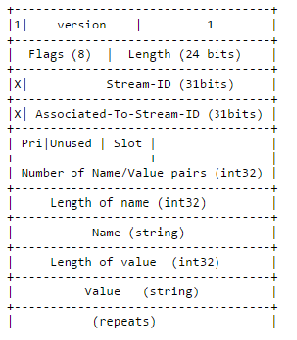
\includegraphics[scale=1]{synstream.png}  %el parámetro scale permite agrandar o achicar la imagen. En el nombre de archivo puede especificar directorios
\centering
\caption{Estructura del control\_frame} \label{fig:figura3}
Permite al remitente crear un stream de forma asíncrona entre los endpoints.
\end{figure}
\begin{itemize}
\item \textbf{Stream-ID:} Un identificador de 31 bits para el stream.
\item \textbf{ID asociado a un stream} Un identificador de 31 bits al cual está asociado. Si el stream es  independiente este valor debería ser 0.
\item \textbf{Prioridad:} 3 bits con la prioridad.
\item \textbf{Sin uso:} 5 bits de espacio sin uso.
\item \textbf{Slot:} 8 bits de un entero sin signo especificando el índice del vector de credenciales del servidor. Si hay un 0 significa que no hay significado a este stream.
\item \textbf{Bloque cabecera nombre/valor} Un nombre o valor para la parte del SYN\_STREAM.
Si el endpoint recibe un SYN\_STREAM 
\end{itemize}
Si un endpoint recibe un SYN\_STREAM que es más grande que los que la implementación soporta, se puede enviar un RST\_STREAM con un FRAME\_TOO\_LARGE. Todas las implementaciones deben soportar los tamaños mínimos.

\subsection{SYN\_REPLY}
\begin{figure}[H] %con el [H] le obligamos a situar aquí la figura
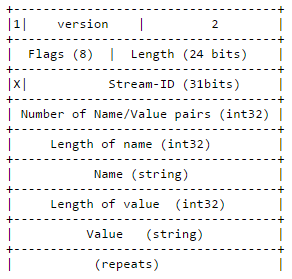
\includegraphics[scale=1]{synreply.png}  %el parámetro scale permite agrandar o achicar la imagen. En el nombre de archivo puede especificar directorios
\centering
\caption{Estructura del SYN\_REPLY} \label{fig:figura4}
\end{figure}
Permite al remitente crear un stream de forma asíncrona entre los endpoints.

Indica la aceptación de una corriente de creación por parte del receptor de un SYN\_STREAM. 
\begin{itemize}
\item \textbf{Stream-ID:} Similar al campo Stream-ID SYN\_STREAM.
Si un endpoint recibe varios SYN\_REPLY por el mismo ID del stream activo, deberá emitir un error de stream con el código STREAM\_IN\_USE. 
\item \textbf{Bloque de cabecera nombre/valor} Similar al campo del mismo nombre del SYN\_STREAM.
\end{itemize}
Si un endpoint recibe un SYN\_REPLY que es más grande que lo que la implementación es capaz de soportar, se puede enviar un RST\_STREAM con el código de error FRAME\_TOO\_LARGE. Todas las implementaciones deben soportar los límites mínimos de tamaño definidos.

\subsection{RST\_STREAM}
\begin{figure}[H] %con el [H] le obligamos a situar aquí la figura
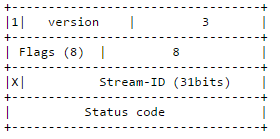
\includegraphics[scale=1]{rststream.png}  %el parámetro scale permite agrandar o achicar la imagen. En el nombre de archivo puede especificar directorios
\centering
\caption{Estructura del RST\_STREAM} \label{fig:figura5}
\end{figure}
Permite la terminación anormal de un stream. Cuando es enviada por el creador de un stream, indica que hay que cancelar el stream. Cuando enviada por el destinatario de una corriente, que indica que hay un error o que el destinatario no quería aceptar el stream, por lo que el stream se cerrará.
\begin{itemize}
\item \textbf{Flags:} RST\_STREAM No usa ningún flag por lo que su valor es 0.
\item \textbf{Longitud:} Puede llegar a tener un tamaño de 24 bits pero en el caso de RST\_STREAM, este valor es siempre 8.

\item \textbf{Stream-ID:} 31 bits que forman la id.
\item \textbf{Status code:} Un indicador de 32 bits para cuando el stream está terminado. 
\\
	\begin{itemize}
    \item \textbf{PROTOCOL\_ERROR:} Error genérico.
    \item \textbf{INVALID\_STREAM:} Cuando el stream no está activo.
    \item \textbf{REFUSED\_STREAM:} El stream fue rechazado antes de que se hiciera ningún proceso.
    \item \textbf{UNSUPPORTED\_VERSION:} Indica que el destinatario de un stream no es compatible con la versión del SPDY solicitado.
    \item \textbf{CANCEL:} Utilizado por el creador de un stream para indicar que el stream ya no es necesario.
    \item \textbf{INTERNAL\_ERROR:} Es un error genérico que puede ser usado cuando la aplicación ha fallado internamente.
    \item \textbf{FLOW\_CONTROL\_ERROR:} Se violó el protocolo de control de flujo.
    \item \textbf{STREAM\_IN\_USE:} El endpoint recibió un SYN\_REPLY para un stream ya abierto.
    \item \textbf{STREAM\_ALREADY\_CLOSED:} El endpoint recibe un stream de datos o SYN\_REPLY de un stream que está medio cerrado.
    \item \textbf{INVALID\_CREDENTIALS:} El servidor recibió una solicitud de un recurso cuyo origen no tiene credenciales válidas en el vector de certificado del cliente.
    \item \textbf{FRAME\_TOO\_LARGE:} El endpoint recibe un stream que la aplicación no puede soportar. Si se envía sin procesar completamente la parte comprimida, el estado de compresión estará fuera de sincronía con el otro endpoint. Entonces el remitente deberá cerrar el stream.
\end{itemize}
\end{itemize}

\subsection{GOAWAY}
\begin{figure}[H] %con el [H] le obligamos a situar aquí la figura
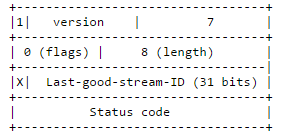
\includegraphics[scale=1]{goaway.png}  %el parámetro scale permite agrandar o achicar la imagen. En el nombre de archivo puede especificar directorios
\centering
\caption{Estructura del GOAWAY} \label{fig:figura6}
\end{figure}
El GOAWAY control\_frame es un mecanismo para decir debe parar de crear stream en la sesion. Este frame de control puede ser enviado por el cliente o el servidor y, una vez enviado el remitente no responderá a ninguna SYN\_STREAM en esta sesión.
\\
\\
Hay que tener en cuenta que algunos servidores optan por enviar el GOAWAY y finalizar inmediatamente la conexión sin esperar que el servidor de streams activos acabe. El cliente será capaz de determinar esto ya que los streams SPDY han terminado de manera abrupta lo que obliga al cliente a decidir si debe reintentar las peticiones pendientes. Los clientes deberán ser capaces de hacer frente a este caso.
Los servidores más novedosos serán capaces de terminar el flujo de stream activo antes de terminar la conexión.
Si un cliente que utilice SPDY cierra la conexión, tambien debería mandar un mensaje GOAWAY.
\\
\\
EL GOAWAY tiene una estructura muy simple, cuenta con:
\begin{itemize}
 \item \textbf{Bit de control.}
 \item \textbf{La version de SPDY.}
 \item \textbf{Tipo.} Siempre es 7 en el caso de GOAWAY.
 \item \textbf{La longitud del frame.} Este es siempre 8 bytes.
 \item \textbf{La ID del último stream respondido.} Consta de 31 bits.
 \item \textbf{Razón por la que se ha cerrado la sesión.}
\end{itemize}

\subsection{SETTINGS}
El frame SETTINGS contiene un conjunto de pares de valores ID/valor para la comunicación de la configuracion de datos sobre como los dos endpoints deben comunicarse.
\\
\\
El marco de SETTINGS puede ser enviado a cualquier momento por cualquier endpoint, su envío es opcional y totalmente asíncrono. Cuando el servidor es el remitente, este puede solicitar la configuración de datos del cliente a través de la sesión de SPDY.

\begin{figure}[H] %con el [H] le obligamos a situar aquí la figura
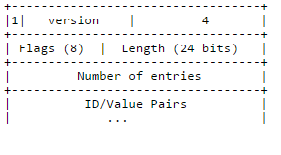
\includegraphics[scale=1]{settings1.png}  %el parámetro scale permite agrandar o achicar la imagen. En el nombre de archivo puede especificar directorios
\centering
\caption{Estructura del SETTINGS} \label{fig:figura7}
\end{figure}

\begin{itemize}
 \item \textbf{Bit de control.}
 \item \textbf{La version de SPDY.}
 \item \textbf{Tipo.} Es siempre es 4 en el caso de SETTINGS.
 \item \textbf{Un flag que puede ser:} FLAG\_SETTINGS\_CLEAR\_SETTING o FLAG\_ SETTINGS\_PERSIST\_VALUE  según si existe o no un par de ID/valor
 \item \textbf{La ID del último stream respondido.} Consta de 31 bits.
 \item \textbf{Una longitud de 24-bit.} El tamaño total de un SETTINGS frame es de 8 bytes + la longitud.
 \item \textbf{Número de entradas.} Un valor de 32-bit que representa el número de pares de ID/valor en el mensaje.
 \item \textbf{Par de ID/valor.}
\end{itemize}

Dentro del par de ID/valor encontramos una subdivisión que consta de:

\begin{figure}[H] %con el [H] le obligamos a situar aquí la figura
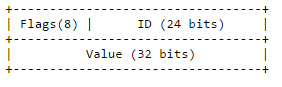
\includegraphics[scale=1]{settings2.png}  %el parámetro scale permite agrandar o achicar la imagen. En el nombre de archivo puede especificar directorios
\centering
\caption{Estructura de la pareja ID/valor} \label{fig:figura8}
\end{figure}

\begin{itemize}
\item \textbf{Un flag que puede ser FLAG\_SETTINGS\_CLEAR\_SETTING o FLAG\_ SETTINGS\_PERSIST\_VALUE} Según si existe o no un par de id/valor, es la misma descrita anteriormente.
\item \textbf{ID (24-bits) :}
 \begin{itemize}
 \item \textbf{SETTINGS\_UPLOAD\_BANDWIDTH:} Permite al remitente enviar el valor máximo de su ancho de banda de subida por este canal. Este número es una estimación.
 \item \textbf{SETTINGS\_DOWNLOAD\_BANDWIDTH:}  Permite al remitente enviar el valor máximo de su ancho de banda de descarga por este canal. Este número es una estimación.
 \item \textbf{SETTINGS\_ROUND\_TRIP\_TIME:} Permite enviar el tiempo mínimo que tarda un control\_ frame en enviarse y recibir respuesta. Este valor se representa en milisegundos.
 \item \textbf{SETTINGS\_MAX\_CONCURRENT\_STREAMS:}  Envía información acerca del máximo número de streams concurrentes inicializados remotamente. No debería ser menor de 100. 
 \item \textbf{SETTINGS\_CURRENT\_CWND:} Permite informar al endpoint remoto sobre el valor TCP CWND.
 \item \textbf{SETTINGS\_DOWNLOAD\_RETRANS\_RATE:} Permite al remitente enviar información acerca de los bytes retransmitidos.
 \item \textbf{SETTINGS\_INITIAL\_WINDOW\_SIZE:} Informa sobre el tamaño de la ventana.
 \item \textbf{SETTINGS\_CLIENT\_CERTIFICATE\_VECTOR\_SIZE:} Nos indica el tamañó del vector certificado de cliente.
\end{itemize}
\end{itemize}

\subsection{PING}
El frame de control PING es un mecanismo de medición del tiempo de ida y vuelta del emisor. Puede ser enviado desde un cliente o un servidor. Los destinatarios del frame de ping deben enviar el mismo frame al emisor tan pronto como sea posible. Cada ping debe utilizar su propio ID.
\begin{itemize}
\begin{figure}[H] %con el [H] le obligamos a situar aquí la figura
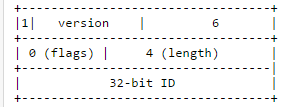
\includegraphics[scale=1]{ping.png}  %el parámetro scale permite agrandar o achicar la imagen. En el nombre de archivo puede especificar directorios
\centering
\caption{Estructura del PING} \label{fig:figura9}
\end{figure}
 \item \textbf{Bit de control.}
 \item \textbf{La versión de SPDY.}
 \item \textbf{Tipo} Siempre es 6 en el caso de PING.
 \item \textbf{La longitud del frame.} Este es siempre 4 bytes.
 \item \textbf{ID:} Es un valor de 32 bits que manda tanto el cliente como el servidor. Tiene una característica especial que se trata de que los usuarios mandan el ping con una ID par, mientras que los servidores con una impar. Esto busca evitar bucles erroneos ya que hay una posibilidad de que tanto el cliente como el servidor manden el ping a la vez. Una vez se han usado todos los IDs (2\^31 posibilidades) se empienzan a reusar las IDs.
\end{itemize}

\subsection{HEADERS}
Los frames HEADERS aumentan los streams con cabeceras adicionales. Este puede ser mandado a un stream ya existente. El bloque de la cabecera formado por nombre/valor está comprimido en este frame.
\\
Tiene la siguiente estructura:

\begin{figure}[H] %con el [H] le obligamos a situar aquí la figura
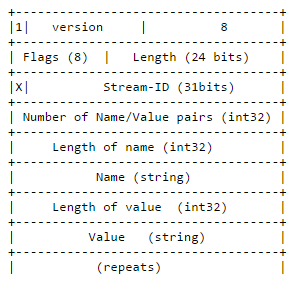
\includegraphics[scale=1]{headers.png}  %el parámetro scale permite agrandar o achicar la imagen. En el nombre de archivo puede especificar directorios
\centering
\caption{Estructura del HEADERS} \label{fig:figura10}
\end{figure}

\begin{itemize}
 \item \textbf{Flags.} El flag válido para este frame es el FLAG\_FIN, este flag indica cual es el último frame que ha sido transmtido por el stream.
  \item \textbf{Longitud.} Tiene 24 bits de longitud, también tiene un valor mínimo es que es 4 bits(0000)
  \item \textbf{Stream-ID.} Es el stream con el que la cabecera está asociada.
  \item \textbf{Nombre/valor de cabecera.} Utiliza el conjunto de pares de nombre/valor que se explica en SYN\_Stream
\end{itemize}

\subsection{WINDOW UPDATE}
El frame de control WINDOW\_UPDATE se usa para controlar la corriente del stream de SPDY.  El control de flujo en SPDY es por salto, es decir, solo entre los dos endpoints de una conexión SPDY. Si hay uno o más intermediarios entre el cliente y el servidor de origen, el flujo de señales de control no se reenvían explícitamente por los intermediarios.Los destinatarios deben poder soportar todos los control\_frames. Si uno destinatario no puede no puede soportarlo deberá emitir un stream error con el código FLOW\_CONTROL\_ERROR.
\\
\\
El control de flujo de SPDY está implementado mediante una ventana de transferencia de datos mantenida por el emisor de cada corriente que indica el número de bytes de datos que el remitente puede transmitir. Después se crea un stream, pero antes de que se haya transmitido algún data\_frame, el remitente comienza con el tamaño de ventana inicial.  Este tamaño de la ventana es una medida de de la capacidad de buffering del destinatario. El remitente no debe enviar un data\_frame mayor que el tamaño de la ventana de transferencia. Después de enviar cada data\_frame, el emisor disminuye su tamaño de la ventana de transferencia por la cantidad de datos transmitidos. Cuando el tamaño de la ventana se hace menor o igual a 0, el remitente debe hacer una pausa en la transmisión de data\_frames. En el otro extremo de la corriente, el receptor envía un WINDOW\_UPDATE para volver a notificar al remitente de que se ha consumido algunos datos y ha liberado espacio de buffering para recibir más datos.
\\
\begin{figure}[H] %con el [H] le obligamos a situar aquí la figura
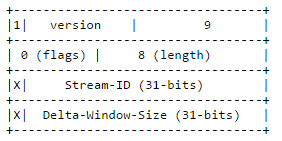
\includegraphics[scale=1]{windowupdate.png}  %el parámetro scale permite agrandar o achicar la imagen. En el nombre de archivo puede especificar directorios
\centering
\caption{Estructura del window update} \label{fig:figura11}
\end{figure}

\begin{itemize}
    \item \textbf{Bit de control:} El bit de control es siempre 1 para este mensaje.
    \item \textbf{Versión:} El número de versión de SPDY.
    \item \textbf{Type:} El tipo de mensaje para un mensaje WINDOW\_UPDATE es 9.
    \item \textbf{Length:} El campo de longitud es siempre 8.
    \item \textbf{Stream-ID:} El ID del stream para el control\_frame WINDOW\_UPDATE.
    \item \textbf{Delta-Window-Size:} El número adicional de bytes que el remitente puede transmitir.
\end{itemize}

\section{Seguridad}
\begin{itemize}
  \item \textbf{El uso de las limitaciones del mismo origen.}
    Esta especificación utiliza la política de mismo origen en todos los casos donde se requiere verificación de contenido.
  \item \textbf{Cabeceras de HTTP y SPDY.}
    A nivel de aplicación , HTTP usa pares de nombre/valor en sus cabeceras.
    \\
    Debido a que PDY fusiona las cabeceras HTTP existentes con las cabeceras SPDY, hay un posibilidad de que algunas aplicaciones HTTP ya usen un nombre particular para la cabecera. 
	\\Para evitar cualquier conflicto, todos los encabezados introducidas por HTTP sobre SPDY están prefijadas con ":".":".  Esto no es una secuencia válida para el nombramiento del encabezado HTTP. 
\item \textbf{Ataques a través de protocolo.}
Mediante la utilización de TLS, SPDY no introduce ningún nuevo protocolo de ataques. TLS cifra los contenidos de todas las transmisiones.
\item \textbf{Subida de encabezados implícitos.}
Subir recursos no tiene ninguna petición asociada. Para poder validar el control de caché existentes todos los recursos almacenados en caché debe tener un conjunto de solicitud de cabeceras. Por esta razón, los navegadores deben tener cuidado con no heredar encabezados de solicitud de la corriente asociada para la subida. 
\end{itemize}

\section{Conclusión}
Como hemos visto SPDY es un protocolo desarrollado objetivamente para conseguir unos objetivos necesarios:
\begin{itemize}
\item Reducir el tiempo de carga de una página. LLegado a conseguir reducirla en alrededor de un 50\%
\item Minimizar la complejidad actual. SPDY utiliza TCP como capa de transporte lo que hace que no requiera cambios en la infraestructura ya existente en la red.
\item Con su estructura consigue que no sea necesario cambiar nada en las web ya creadas.
\item Utiliza el código abierto consiguiendo la ayuda de la comunidad y especialistas en la industria.
\end{itemize}
Algunas de las ventajas técnicas que nos ofrece SPDY son:

\begin{itemize}
\item Permitir que muchas peticiones HTTP que ocurren de manera concurrente pasen a través de una sola sesión TCP.
\item Reduce el ancho de banda utilizado actualmente por HTTP mediante la compresión de cabeceras y la eliminación de las que no son necesarias.
\item Es un protocolo muy fácil de implementar y eficiente a nivel de servidor. HTTP tenía el inconveniente de ser demasiado complejo.
\item Hace el protocolo de transporte SSL mucho más seguro y compatible a las infraestructuras existentes en internet. Además, SSL introduce la penalización de la latencia y es necesario para asegurar que la comunicación a través de los proxies no se ha roto.
\item Permite que el servidor inicie comunicaciones con el cliente y envíe los datos a este cuando sea posible.
\end{itemize}

\bibliographystyle{unsrt}
\begin{thebibliography}{a}
\bibitem{1}
\url{https://docs.google.com/a/chromium.org/viewer?a=v&pid=sites&srcid=Y2hyb21pdW0ub3JnfGRldnxneDoxMzcyOWI1N2I4YzI3NzE2}

\bibitem{2} 
\url{https://developers.google.com/speed/protocols/}
 
\bibitem{3}
\url{https://www.chromium.org/spdy/spdy-whitepaper}

\bibitem{4} 
\url{https://gist.github.com/anonymous/2011946}

\bibitem{5}
\url{https://wiki.mozilla.org/Platform/Features/SPDY}

\bibitem{6}
\url{https://es.wikipedia.org/wiki/Transmission_Control_Protocol}

\bibitem{7}
\url{http://dev.chromium.org/spdy/spdy-protocol}

\end{thebibliography}
\end{document}
